\documentclass[tikz,border=8pt]{standalone}
\usepackage{amsmath,amssymb}
\usetikzlibrary{calc,arrows.meta,patterns.meta}
% PROFILE-GEOMETRY-V3 — publication geometry authority
\definecolor{Power}{HTML}{C8102E}
\definecolor{Transport}{HTML}{16823A}
\definecolor{Information}{HTML}{1D4ED8}
\definecolor{InterfaceAccent}{RGB}{45,143,214}
\definecolor{InterfaceText}{RGB}{40,120,205}
\definecolor{Violet}{HTML}{6D28D9}
\definecolor{Critical}{HTML}{CF222E}
\definecolor{Ink}{HTML}{1E2933}
\definecolor{Line}{HTML}{E0E5EA}

\newcommand{\regpoly}[5]{%
  \draw[#5,line join=round]
  \foreach \j in {0,...,#1} {
    \ifnum\j=0
      ($(#2)+({#4*cos(90+360*\j/#1)},{#4*sin(90+360*\j/#1)})$)
    \else
      -- ($(#2)+({#4*cos(90+360*\j/#1)},{#4*sin(90+360*\j/#1)})$)
    \fi
  };
}

\begin{document}
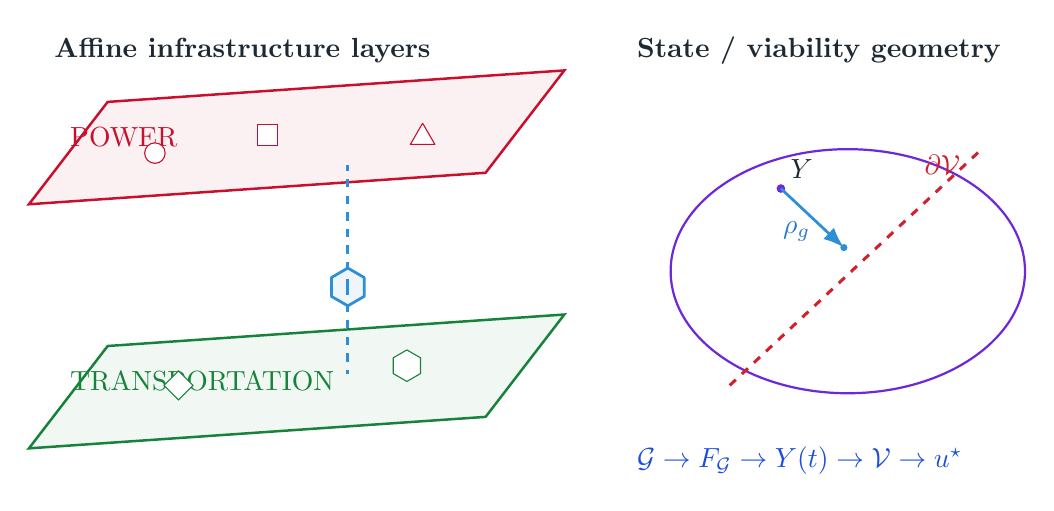
\begin{tikzpicture}[x=1cm,y=1cm,>=Latex,every node/.style={text=Ink}]
  % Affine Power and Transportation planes.
  \fill[Power!6] (0.6,4.5)--(6.4,4.9)--(7.4,6.2)--(1.6,5.8)--cycle;
  \draw[Power,line width=.9pt] (0.6,4.5)--(6.4,4.9)--(7.4,6.2)--(1.6,5.8)--cycle;
  \fill[Transport!6] (0.6,1.4)--(6.4,1.8)--(7.4,3.1)--(1.6,2.7)--cycle;
  \draw[Transport,line width=.9pt] (0.6,1.4)--(6.4,1.8)--(7.4,3.1)--(1.6,2.7)--cycle;

  \node[anchor=west,font=\bfseries] at (0.8,6.45) {Affine infrastructure layers};
  \node[anchor=west,text=Power] at (1.0,5.35) {POWER};
  \node[anchor=west,text=Transport] at (1.0,2.25) {TRANSPORTATION};

  % Typed nodes and shared interface.
  \draw[Power,fill=white] (2.2,5.15) circle (.13);
  \draw[Power,fill=white] (3.5,5.25) rectangle +(0.26,0.26);
  \regpoly{3}{5.6,5.35}{unused}{.18}{Power,fill=white}
  \regpoly{6}{4.65,3.45}{unused}{.24}{InterfaceAccent,fill=InterfaceAccent!8,line width=1pt}

  \draw[Transport,fill=white,rotate around={45:(2.5,2.2)}] (2.37,2.07) rectangle (2.63,2.33);
  \regpoly{6}{5.4,2.45}{unused}{.20}{Transport,fill=white}
  \draw[InterfaceAccent,dashed,line width=1pt] (4.65,3.45)--(4.65,5.0);
  \draw[InterfaceAccent,dashed,line width=1pt] (4.65,3.45)--(4.65,2.35);

  % Viability geometry.
  \node[anchor=west,font=\bfseries] at (8.2,6.45) {State / viability geometry};
  \draw[Violet,line width=.8pt] (11.0,3.65) ellipse (2.25 and 1.55);
  \draw[Critical,dashed,line width=1.1pt] (9.5,2.2)--(12.7,5.2);
  \fill[Violet] (10.15,4.7) circle (.055) node[above right] {$Y$};
  \draw[InterfaceAccent,->,line width=1pt] (10.15,4.7)--(10.95,3.95);
  \fill[InterfaceAccent] (10.95,3.95) circle (.045);
  \node[text=InterfaceText] at (10.35,4.15) {$\rho_g$};
  \node[text=Critical] at (12.2,5.0) {$\partial\mathcal V$};

  \node[anchor=west,text=Information] at (8.2,1.25)
    {$\mathcal G\rightarrow F_{\mathcal G}\rightarrow Y(t)\rightarrow\mathcal V\rightarrow u^\star$};
\end{tikzpicture}
\end{document}
